\documentclass[../Differential Equations.tex]{subfiles}

\begin{document}
	\section{Definitions and Terminology}
		\subsectionb{A Definition}
				\callout{17}{\paragraph{Differential Equation}
						An equation containing the derivatives of one or more unknown functions (or dependent variables) with respect to one or more independent variables is a \textbf{differential equation (DE)}.
				}
		\subsectionb{Classification by Type}
			A differential containing only ordinary derivatives with respect to a \textit{single} independent variables is an \textbf{ordinary differential equation (ODE)}. One involving partial derivatives is a \textbf{partial differential equation (PDE)}.
		\subsectionb{Notation}
			\textbf{Leibniz notation} denotes derivatives as ratios of differentials with the operators and variables raised to the \(n\) for the \(n^\th\) derivative.
			\textbf{Prime notation} denotes the \(n^\th\) derivative with either \(n\) primes or \((n)\) in superscript of the dependent variable or the function. The \(n^\th\) derivative of $y = f(x)$ can thusly be denoted as
				\[\dv[n]{y}{x} = y^{(n)} = f^{(n)}(x)\]
			Newton's \textbf{dot notation} is sometimes used to denote derivatives with respect to time, placing \(n\) dots above the dependent variable to denote its \(n^\th\) derivative with respect to \(t\). The second derivative of \(x\) with respect to \(t\) can be denoted as
				\[\ddot{x} = \dv[2]{x}{t}\]
			\textbf{Subscript Notation} is often used for partial derivatives, indicating the independent variable in the subscript. The second partial \(x\) derivative with respect to \(z\) can be denoted as
				\[z_{xx} = \pdv[2]{z}{x}\]
		\subsectionb{Classification by Order}
			The \textbf{order of a differential equation} is the order of the highest derivartive in the equation. \\
			A first-order ODE is sometimes written in the \textbf{differential form}
				\[M(x, y)\dd{x} + N(x, y)\dd{y} = 0\]
			Symbolically, an \(n^\th\)-order ODE in one dependent variable can be expressed generally as
				\[F\bigl(x, y, y', \ldots, y^{(n)}\bigr) = 0\]
				where \(F\) is a real-valued function of \(n + 2\) variables. \\
			It is assumed that it is possible to solve an ODE in the form above uniquely for the highest derivative \(y^(n)\) in terms of the remaining \(n + 1\) variables. \\
			The \textbf{normal form} of the above expression is
				\[\dv[n]{y}{x} = f\bigl(x, y, y', \ldots, y^{(n - 1)}\bigr)\]
				where \(f\) is a real-values continuous function. \\
			The following normal forms can be used to represent general first- and second-order ODEs:
				\begin{align*}
					\dv{y}{x} &= f(x, y)
							& \dv[2]{y}{x} &= f(x, y, y') 
				\end{align*}
		\subsectionb{Classification by Linearity}
			An general \(n^\th\) order ODE is \textbf{linear} if \(F\) is linear in \(y, y', y^{(n)}\). This means that it is linear when
				\[a_n(x)\dv[n]{y}{x} + a_{n - 1}(x)\dv[n - 1]{y}{x} + \cdots + a_1(x)\dv{y}{x} + a_0(x)y = g(x)\]
			Two important special cases of the above are linear first-\footnote{
					A first order ODE written in differential form as \(M(x, y)\dd{x} + N(x, y)\dd{y} = 0\) may be linear or nonlinear, as there is no indication of which symbol is the dependent variable.
				} and second-order DEs:
				\begin{align*}
					a_1(x)\dv{y}{x} + a_0(x)y &= g(x)
							& a_2(x)\dv[2]{y}{x} + a_1(x)\dv{y}{x} + a_0(x)y = g(x)
				\end{align*}
			The characteristic properties of linear ODEs are that the dependent variable and all of its derivatives are of first degree and that the coefficients of those terms are dependent at most on the independent variable. \\
			A \textbf{nonlinear} ODE is one that is not linear. \\
			Nonlinear functions of the dependent variable cannot appear in linear ODEs. \\
			A DE can not be classified as linear or nonlinear if both differentials are in the numerator.
		\subsectionb{Solutions}
			\callout{17}{\paragraph{Solution of an ODE}
				Any function \(\varphi\) defined on an interval \(I\) with at least \(n\) derivatives that are continuous on \(I\) which when substituted into an \(n^\th\)-order ODE reduce the equation to an identity is a \textbf{solution} of the equation on the interval.
			}
			A DE need not have a solutions.
			A solution of a DE may involve \textbf{integral-defined function}\footnote{
					A function \(F\) of a single variable \(x\) can be defined as
						\[F(x) = \int_a^x g(t)\dd{t}\]
						If the integrand \(g\) is continuous over \([a, b]\) and \(x\) falls within the interval, then \(F\) is differentiable on the open interval and
						\[F'(x) = \dv{x}\int_a^x g(t)\dd{t} = g(x)\]
						The integral is often \textbf{nonelementary}, meaning that it is not composed of elementary functions. \\
						Elementary functions include constant, polynomial, rational, exponential, logarithmic, trigonometric, and inverse trigonometric functions, as well as rational powers and finite combinations using the four basic arithmetic operations and compositions of these functions.
				}. \\
			A solution of a general \(n^\th\)-order ODE is a function \(\varphi\) with at least \(n\) derivatives for which
				\[F\bigl(x, \varphi(x), \varphi'(x), \ldots, \varphi^{(n)}(x)\bigr) = 0 \qquad \forall\,x \in I\]
			\(\varphi\) is said to \textit{satisfy} the differential equation on \(I\). It is assumed that a solution \(\varphi\) is a real-valued function. \\
			A solution is occasionally denoted alternatively by \(y(x)\).
		\subsectionb{Interval of Definition}
			The interval \(I\) over which \(\varphi\) satisfies the ODE is referred to as the \textbf{interval of definition/}\hspace{-5pt} \textbf{existence/validity}  or the \textbf{domain of the solution}. \\
			A solution of a DE that is identically 0 on an interval \(I\) is said to be a \textbf{trivial solution}.
		\subsectionb{Solution Curve}
			The graph of \(\varphi\) is called a \textbf{solution curve}. \\
			The domain of \(\varphi\) need not be the same as \(I\).
		\subsectionb{Explicit and Implicit Solutions}
			A function that expresses the dependent variable solely in terms of the independent variable and constants is said to be \textit{explicit}. An \textbf{explicit solution} is a solution with an explicit function. It can be thought of as an explicit formula \(y = \varphi(x)\) that can be manipulated. \\
			An explicit solution is generally not needed over an implicit one. \\
			An implicit solution \(G(x, y) = 0\) may define a differentiable function that is a solution of a DE despite \(G(x, y) = 0\) potentially not being solvable analytically. The solution curve may be a segment of the graph of \(G(x, y) = 0\).
		\subsectionb{Families of Solutions}
			When solving a first-order DE, the solution \textit{usually} contains a single constant or parameter \(C\), similar to the constant of integration obtained from the indefinite integral. A solution of \(F(x, y, y') = 0\) containing constant \(C\) is a set of solutions \(G(x, y, C) = 0\) called a \textbf{one-parameter family of solutions}. \\
			An \(n^\th\)-order DE\footnote{
					\(F\bigl(x, y, y', \ldots, y^{(n)}\bigr) = 0\) may not always be solvable for \(y^{(n)}\).
				} often yields an \textbf{\(\bm{n}\)-parameter family of solutions}\footnote{
					If \textit{every} solution of an \(n^\th\)-order ODE on an interval can be found by manipulating the parameters of an \(n\)-parameter family of solutions, then the family is said to be the \textbf{general solution} of the DE. \\
					Nonlinear ODEs are often difficult of impossible to solve in terms of elementary functions, so if a family of solutions is found for one, it is unclear whether it is a general solution. Practically, the designation of \enquote{general solution} is only given for solutions to linear ODEs.
				} \(G(x, y, C_1, C_2, \ldots, C_n) = 0\). \\
			The parameters in a family of solutions are \textit{arbitrary} up to a point, but they should always take on values that make sense in the real-number system. \\
			A \textbf{singular solution} is one that cannot be obtained by specializing \textit{any} of the parameters in the family of solutions.
		\subsectionb{Systems of Differential Equations}
			A \textbf{system of ODEs} is comprised of multiple unknown functions of a single independent variable. \\
			A \textbf{solution} of a system is a pair of differentiable functions defined on common interval \(I\) that satisfy each equation of the system on the interval.
	\section{Initial-Value Problems}
		Often, a solution to a DE must meet other conditions imposed on it and its derivatives. \\
			\[\dv[n]{y}{x} = f\bigl(x, y, y', \ldots, y^{(n - 1)}\bigr) \mid y(x_0) = y_0, y'(x) = y_1, \ldots, y^{(n - 1)}(x_0) = y_{n - 1}\]
			If these desired values are constants, this is an \textbf{\(\bm{n^\th}\)-order initial-value problem (IVP)}. The desired values are called \textbf{initial conditions (IC)}.\footnote{
					If conditions are prescribed at multiple points, called \textbf{boundary conditions}, the problem is called a \textbf{boundary-value problem (BVP)}.
				} \\
		Solving an \(n^\th\)-order IVP often requires that an \(n\)-parameter family of solutions be found that can then be used in tandem with the constraints to find the constants. The resulting particular solution is defined on some interval that contains \(x_0\).
		\subsectionb{Geometric Interpretation}
			A first-order IVP
				\[\dv{y}{x} = f(x, y) \mid y(x_0) = y_0\]
				can be interpreted as finding a solution \(y(x)\) with a graph that passes through the point \((x_0, y_0)\). \\
			A second-order IVP
				\[\dv[2]{y}{x} = f(x, y, y') \mid y(x_0) = y_0, y'(x_0) = y_1\]
				can be interpreted as finding a solution \(y(x)\) with a graph that passes through \((x_0, y_0)\) with slope \(y_1\).
		\subsectionb{Existence and Uniqueness}
			It can be assumed that \textit{most} DEs will hav solutions and that the solutions of IVPs will \textit{generally} be unique. \\
			\callout{17}{\paragraph{Theorem 1.2.1}
				Let \(R\) be a rectangular region in the \(xy\)-plane defined by
					\[R = \{(x, y) \mid a \le x \le b, c \le y \le d\}\]
					that contains point \((x_0, y_0)\). If \(f(x, y)\) and \(\pdv*{f}{y}\) are continuous over \(R\)\footnote{
							These conditions are sufficient but not necessary. When \(f(x, y)\) and \(\pdv*{f}{y}\) are continuous on \(R\), a solution of the IVP exists and is unique so long as \((x_0, y_0)\) is contained within \(R\). If these conditions are not met, though, the IVP \textit{may} still have a solution that \textit{may} be unique, or it may have multiple or no solutions.
						}, then there exists some interval \(I_0: (x_0 - h, x_0 + h)\) (where \(h > 0\)) contained in \([a, b]\) and a unique function \(y(x)\) defined on this interval that is a solution of the IVP.
			}
		\subsectionb{Interval of Existence/Uniqueness}
			The domain of the function that represents a solution to an IVP, the interval \(I\) over which the solution is defined or exists, and the interval \(I_0\) of existence \textit{and} uniqueness. \\
			Suppose \((x_0, y_0)\) is a  point in the interior of rectangle \(R\). The continuity of function \(f(x, y)\) on \(R\) is sufficient to guarantee the existence of at least on solution of \(\dv*{y}{x} = f(x, y)\), \(y(x_0) = y_0)\), defined on some interval \(I\). The interval of definition \(I\) for this IVP is generally taken to be the largest interval containing \(x_0\) over which the solution \(y(x)\) is both defined and differentiable. The interval depends both on the DE and the initial condition. \\
			The condition of continuity of \(\pdv*{f}{y}\) on \(R\) means that the solution on \(I_0\) containing \(x_0\) is the \textit{only} solution satisfying the initial condition. \\
			It should be noted that the interval of definition \(I\) may not be as wide as \(R\) and the interval of existence \(I_0\) and uniqueness may not be as large as \(I\). The number \(h > 0\) that defines \(I_0\) may be very small, so the solution \(y(x)\) should bed thought of as \textit{unique locally}: a solution defined near \((x_0, y_0)\).
	\section{Differential Equations as Mathematical Models}
		\subsectionb{Mathematical Models}
			A \textbf{mathematical model} is a mathematical description of some system or phenomenon. \\
			To construct a mathematical model, one must first identify the independent variables of the system. The model's \textbf{level of resolution} is determined by which variables are chosen to be included From there, a set of hypotheses about the system can be made. These will include any empirical laws that may apply. \\
			Assumptions made regarding a system often involve \textit{rates of change}, so their models often include \textit{derivatives}; that is to say, mathematical models often take the form of DEs or system of them. \\
			If the DE or system is solvable, then the model can be considered reasonable if the solution is in line with data or known facts. Otherwise, the level of resolution can be increased or alternative assumptions can be made.
			\callout{15}{\paragraph{Steps in the modeling process with differential equations}
				\[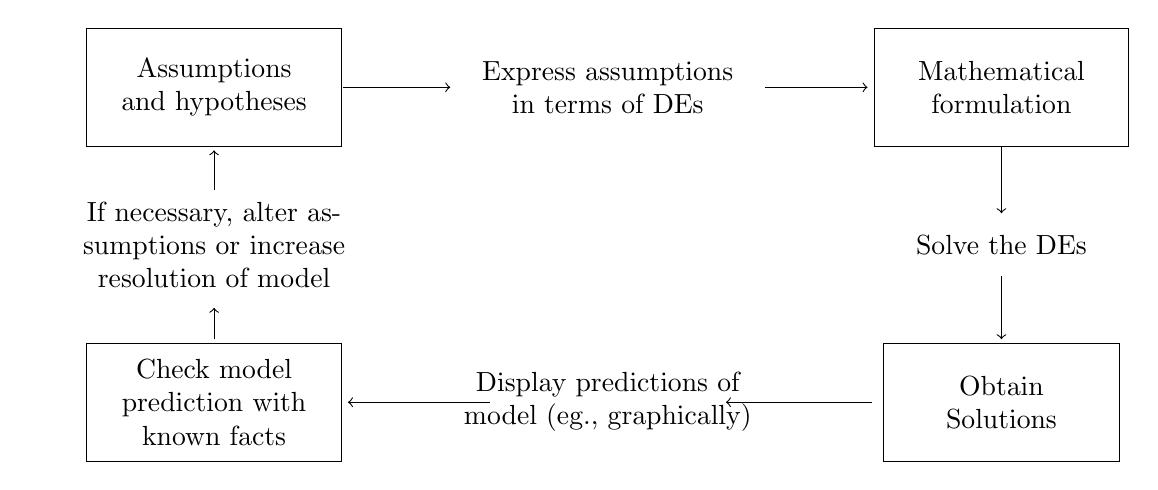
\begin{tikzpicture}[yscale = 2]
					\node at (-5, 1) [draw, minimum height = 1.5 cm, minimum width = 3cm, align = center, text width = 3cm] {Assumptions and hypotheses};
						\draw[->] (-3.36, 1) -- (-2, 1);
					\node at (0, 1) [align = center, text width = 4cm] {Express assumptions in terms of DEs};
						\draw[->] (2, 1) -- (3.3, 1);
					\node at (5, 1) [draw, minimum height = 1.5cm, minimum width = 3cm, align = center, text width = 3cm] {Mathematical formulation};
						\draw[->] (5, 0.625) -- (5, 0.2); 
					\node at (5, 0) [align = center] {Solve the DEs};
						\draw[->] (5, -0.2) -- (5, -0.6);
					\node at (5, -1) [draw, minimum height = 1.5cm, minimum width = 3cm, align = center, text width = 2cm] {Obtain Solutions};
						\draw[->] (3.36, -1) -- (1.5, -1);
					\node at (0, -1) [align = center, text width = 4cm] {Display predictions of model (eg., graphically)};
						\draw[->] (-1.5, -1) -- (-3.3, -1);
					\node at (-5, -1) [draw, minimum height = 1.5cm, minimum width = 3cm, align = center, text width = 3cm] {Check model prediction with known facts};
						\draw[->] (-5, -0.6) -- (-5, -0.4);
					\node at ( -5, 0) [align = center, text width = 4.5cm] {If necessary, alter assumptions or increase resolution of model};
						\draw[->] (-5, 0.35) -- (-5, 0.6);
				\end{tikzpicture}\]
			}
			Increasing the resolution also increases the complexity of the model, meaning that an explicit solution becomes less likely. \\
			Mathematical models of physical systems often involve time as a variable \(t\). A solution gives the \textbf{state of the system}.
		\subsectionb{Population Dynamics}
			The \textbf{Malthusian model for population growth} assumes that the the growth rate over a certain time is proportional to the total population at that time.
				\[\dv{P}{t} \propto P \qquad \text{or} \qquad \dv{P}{t} = kP\]
				Due to its simplicity, it is only used to model the \textit{growth of small populations over short intervals}. \\
				This model is also used for the model of continuous compound interest \(\dv*{S}{t} = rS\) (where \(S\) is capital and \(r\) is the annual interest rate).
		\subsectionb{Radioactive Decay}
			\textbf{Radioactive decay} can be modeled under the assumption that the rate \(\dv*{A}{t}\) at which a substance's nuclei decay is proportional to the number of nuclei \(A(t)\) of the substance remaining at time \(t\).
				\[\dv{A}{t} \propto A \qquad \text{or} \qquad \dv{A}{t} = kA\]
			This model is also used to determine a drug's half-life and in the model of a first-order chemical reaction.
			\callout{15.33}{
				\textit{A single differential equation may serve as a mathematical model for many phenomena.}
			}
			Mathematical models often have side conditions, meaning that they may either be IVPs or BVPs.
		\subsectionb{Newton's Law of Warming/Cooling}
			Newton's law of cooling/warming can be expressed as 
				\[\dv{T}{t} \propto T - T_m \qquad \text{or} \qquad \dv{T}{t} = k(T - T_m)\]
				where \(T\) is temperature of the body, \(T_m\) is the temperature of the surrounding medium, and \(t\) is time.
		\subsectionb{Spread of a Disease}
			The spread of a disease can be modeled as
				\[\dv{x}{t} = kxy\]
				where \(x(t)\) is the number of people that have contracted the disease and \(y(t)\) is the number of people that have not been exposed. The product of these two can be used to approximate the number of interactions between the two groups.
		\subsectionb{Chemical Reactions}
			Radioactive decay is a \textbf{first-order reaction}. Such a reaction can be modeled as
				\[\dv{X}{t} = kX\]
				where \(X(t)\) is the amount of substance \(A\) remaining. \\
			Suppose one molecule each of substances \(A\) and \(B\) is used to form a single molecule of substance \(C\). If \(X\) is the amount of \(C\) formed and \(\alpha\) and \(\beta\) are the initial amounts of \(A\) and \(B\), then the instantaneous amounts of \(A\) and \(B\) that have not yet been converted are \(\alpha - X\) and \(\beta - X\) respectively. The rate of formation of \(C\) is therefore given by
				\[\dv{X}{t} = k(\alpha - X)(\beta - X)\]
				A reaction modeled by this is said to be a \textbf{second-order reaction}
		\subsectionb{Mixtures}
			If \(A(t)\) denotes the amount of salt at time \(t\), then the rate at which this changes is
				\[\dv{A}{t} = R_{\text{in}} - R_{\text{out}}\]
		\subsectionb{Draining a Tank}
			\textbf{Torricelli's law} states that the speed \(v\) of efflux of water through a sharp-edged hole at the bottom of a container filled to depth \(h\) is equal to the speed that a body would acquire in free fall from the same height (\(v = \sqrt{2gh}\) where \(g\) is acceleration due to gravity). If the are of the hole is \(A_h\) and the speed of water leaving is \(v = \sqrt{2gh}\), then the volume of water leaving per second is \(A_h\sqrt{2gh}\). If \(V(t)\) denotes the volume of water remaining at time \(t\), then
				\[\dv{V}{t} = -A_h\sqrt{2gh}\]
		\subsectionb{Series Circuits}
			Consider the \textit{LRC}-series circuit
				\[\begin{circuitikz}[xscale = 2, yscale = 1.5]
					\draw (0, 0)
						to[V = $E(t)$] (0, 2)
						to[L = $L$] (2, 2)
						to[R = $R$] (2, 0)
						to[C = $C$] (0, 0);
				\end{circuitikz}\]
\end{document}